\section{Mediciones}

Se realizaron mediciones en base a crear sets de distinta cantidad de
elementos, con la cantidad de subsets y la cantidad de elementos por subset
siendo proporcional a la cantidad de elementos.

Para asegurar la validez de las comparaciones todas las mediciones fueron
realizadas sobre los mismos sets de datos para los m\'etodos que est\'an siendo
comparados. Los elementos fueron generados por los valores pseudoaleatorios del
lenguaje (el m\'odulo \texttt{random}) con la misma \textit{seed}.

\subsection{Backtracking vs. Programación Lineal}

\begin{figure}[H]
    \centering
    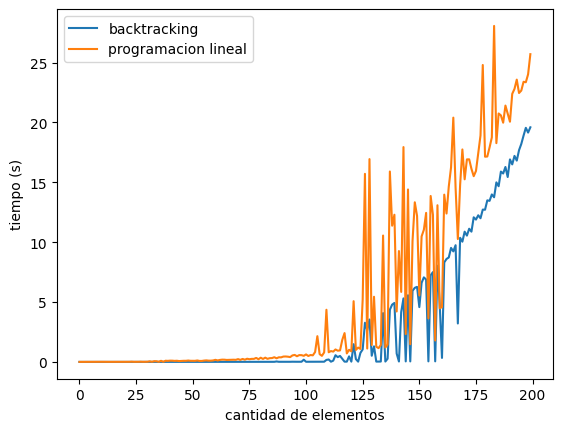
\includegraphics[width=1\textwidth]{img/backvslp.png}
\end{figure}

Backtracking obtiene mejores tiempo de ejecución que programación lineal para
encontrar la solución óptima.

\subsection{Algoritmos de aproximaci\'on}

\begin{figure}[H]
    \centering
    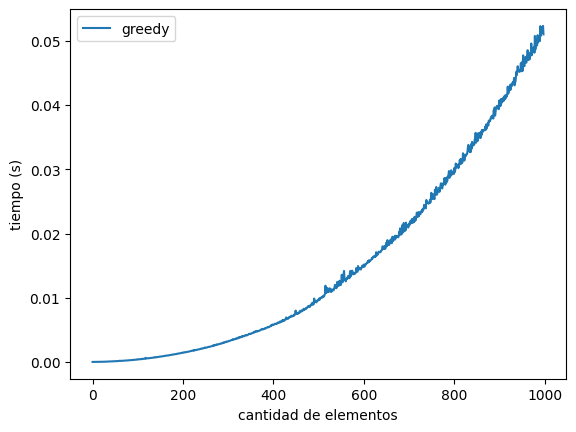
\includegraphics[width=0.49\textwidth]{img/greedy.png}
    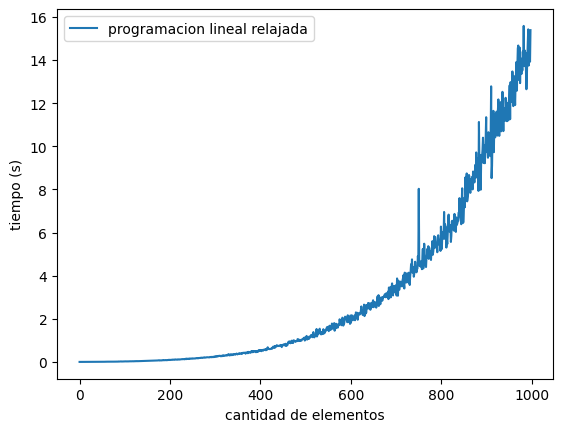
\includegraphics[width=0.49\textwidth]{img/pl_rlx.png}
\end{figure}

Notar la diferencia de tiempos (eje y) entre greedy y programación lineal.
